
\section{Ejercicio 8: Dise\~no de controlador para un Joystick Anal\'ogico}\subsection{Introducci\'on}
En esta secci\'on se realiza el dise\~no e implementaci\'on de un circuito que permite sensar la posici\'on de un joystick en un determinado eje, y mostrarla de forma num\'erica, entre 0 y 99, en un display con refresco variable desde 1Hz a 20Hz. Para llevar a cabo esta tarea se divide al sistema en varios m\'odulos, acorde a las funciones que estos cumplen.

Ademas, se presentan las simulaciones y razonamientos te\'oricos correspondientes a cada m\'odulo, que respaldan el dise\~no realizado.

\subsection{Dise\~no}
Para realizar el dise\~no se parte del diagrama en bloques que se presenta en la Figura \ref{fig:BLOCK_DIAG}. 
\begin{figure}[H]
    \centering
    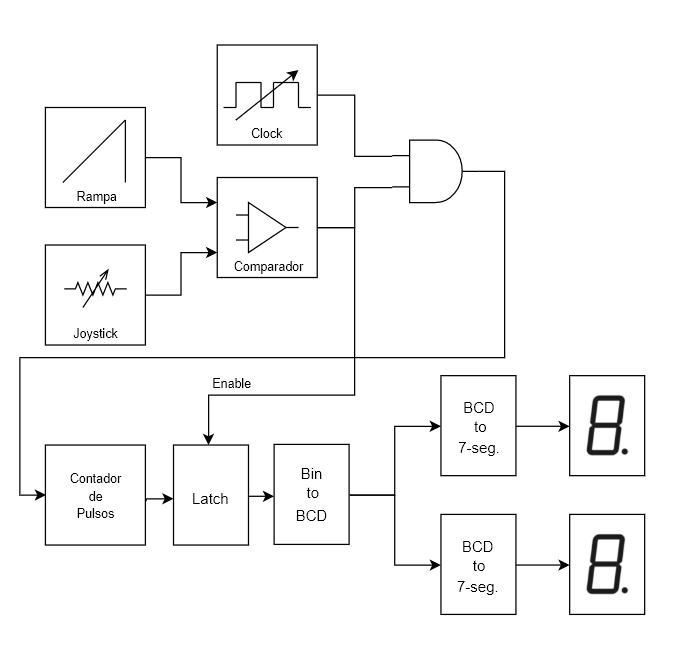
\includegraphics[width=0.9\textwidth]{../EJ8/Recursos/flowDiagram.png}
    \caption{Diagrama en bloques del sistema}
    \label{fig:BLOCK_DIAG}
\end{figure}
A partir de este diagrama es posible ver el funcionamiento general del sistema, as\'i como tambi\'en el conexionado entre los m\'odulos que lo componen.

En cuanto al dise\~no f\'isico de los PCB, se decide separar el sistema en sus m\'odulos del diagrama en bloques por dos razones principales. la primera es la f\'acil localizaci\'on de problemas de funcionamiento, debido a que es posible probar las etapas por separado antes de conectarlas en su totalidad. La segunda es la clara distinci\'on y separaci\'on de circuitos anal\'ogicos y digitales, lo que minimiza la interferencia entre ellos 

En las siguientes secciones se describe com mayor profundidad el dise\~no de cada uno de los m\'odulos por separado.


\subsubsection{Generador de rampa y comparador (ADC)}
En el dise\~no de esta etapa se parte de la base de que se requiere convertir la tensi\'on continua que se obtiene del joystick, se comporta como un divisor resistivo variable, en una se\~nal digital que sea posible dimensionar y mostrar en los displays.
Para implementar este circuito se decide utilizar un conversor que se basa en el concepto de conversor A/D de rampa simple. La principal caracter\'istica de este tipo de conversores es que, la se\~nal a convertir, necesariamente una una tensi\'on continua, es comparada con una se\~nal de tipo rampa.
luego se cuentan pulsos hasta que la rampa cruza ene nivel de tensi\'on y en base a la cantidad de pulsos contados puede saberse el valor de la tensi\'on a la entrada.

Se muestra en la Figura \ref{fig:CIRCUIT_RAMP}  el esquem\'atico completo utilizado, que consta de un generador de rampa y un comparador. 
\begin{figure}[H]
    \centering
    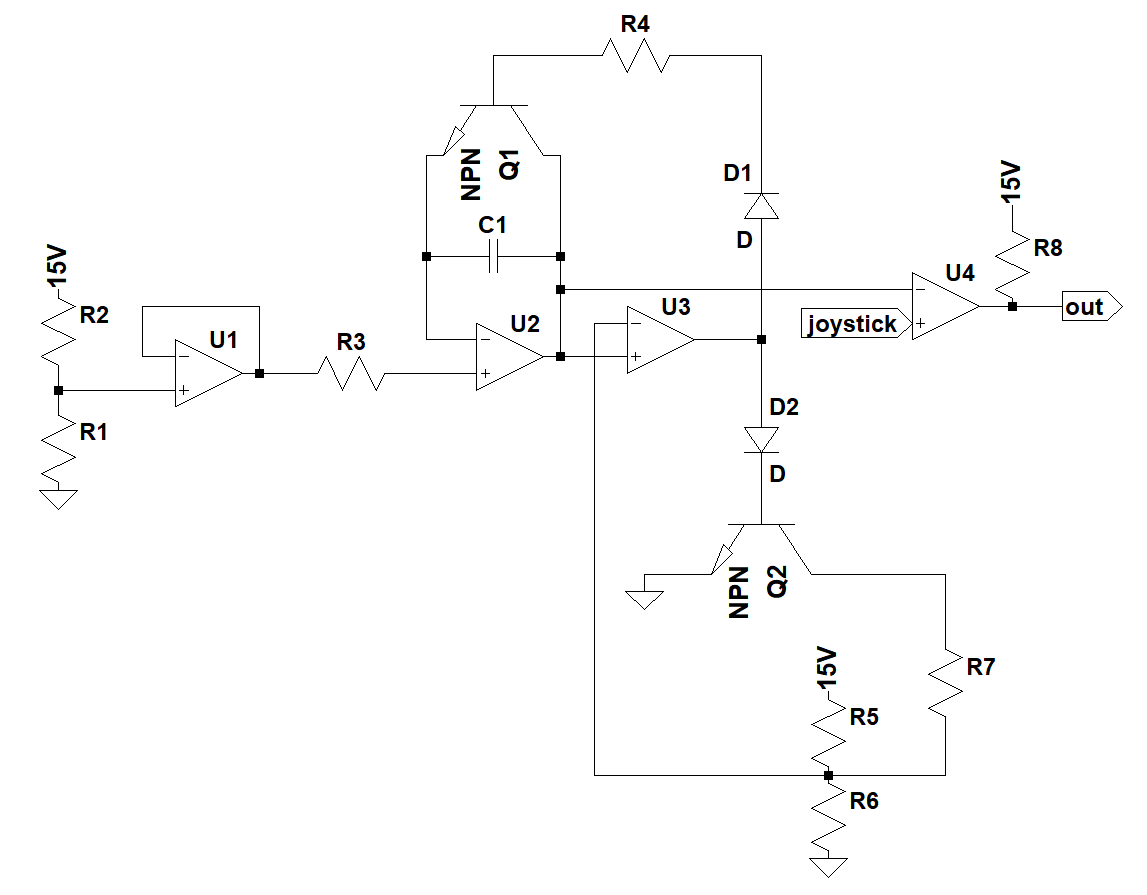
\includegraphics[width=0.9\textwidth]{../EJ8/Recursos/analogCircuit.png}
    \caption{Circuito esquem\'atico del comparador de rampa simple}
    \label{fig:CIRCUIT_RAMP} 
\end{figure}


El circuito es,por su naturaleza, un VCO (\textit{Voltage Controlled Oscillator}). La forma en que funciona es, se fija la tensi\'on sobre la resistencia R1 de $100k \Omega$, en un nodo utilizando al buffer y en el otro debido a la \textit{masa virtual} del amplificador operacional U2. Esto forma una fuente de corriente regulable por la tensi\'on a la entrada. Es imporante la utilizacion de el buffer para que la corriente que circula en el circuito, no afecte al divisor resistivo y pueda seguirse considerando que se cumple la ecuaci\'on que lo describe $\frac{V_o}{V_i} = \frac{R_2}{R_1+R_2}$

Esta corriente constante es integrada con el amplificador operacional U4, para lograr una tensi\'on que aumenta linealmente. 

Para lograr el flanco descendente de la rampa se compara la tensi\'on con un nivel de continua que controla la amplitud de la se\~nal de salida, y tambi\'en modifica significativamente su frecuencia. Cuando coinciden el operacional U3, que esta funcionando como comparador, provoca que que los transistores pasen de corte a saturaci\'on lo que hace que el capacitor se descargue y adem\'as fuerza 0V en la entrada no inversora de U3 lo que permite que su salida vuelva a 0V y el proceso vuelva a comenzar.

Finalmente se utiliza, para comparar la tensi\'on del joystick con la rampa un circuito integarado comparador, el LM311, que al tener una salida \textit{Open Collector} permite obtener una salida digital para el DAC. Esta es posteriormente utilizada para detener la cuenta y obtener la posic\'on del joystick.

Se agrega, adem\'as, la salida RESET, que se utiliza para reiniciar la cuenta una vez que la rampa se reinicia.

Se puede observar en la Figura \ref{fig:DAC} las diferentes se\~nales que se observan en el DAC, que permiten comprender el funcionamiento del mismo.

\begin{figure}[H]
    
    \centering
    \begin{tabular}{c c}
        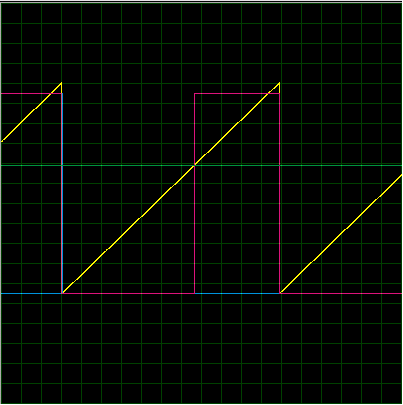
\includegraphics[width=0.4\textwidth]{../EJ8/Recursos/OSC_DAC} &
        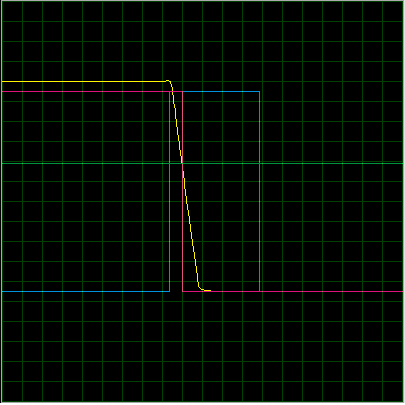
\includegraphics[width=0.4\textwidth]{../EJ8/Recursos/OSC_DAC_RST}
    \end{tabular}
    \caption{Se\~nales de inter\'es a la salida del DAC. Generador de rampa en amarillo, joystick en verde, salida del comparador en rosa y RESET en azul }
    \label{fig:DAC}
\end{figure}

Por ultimo se muestra en la Figura \ref{fig:PCB_ANALOG} el PCB utilizado para las pruebas.
\begin{figure}[H]
    \centering
    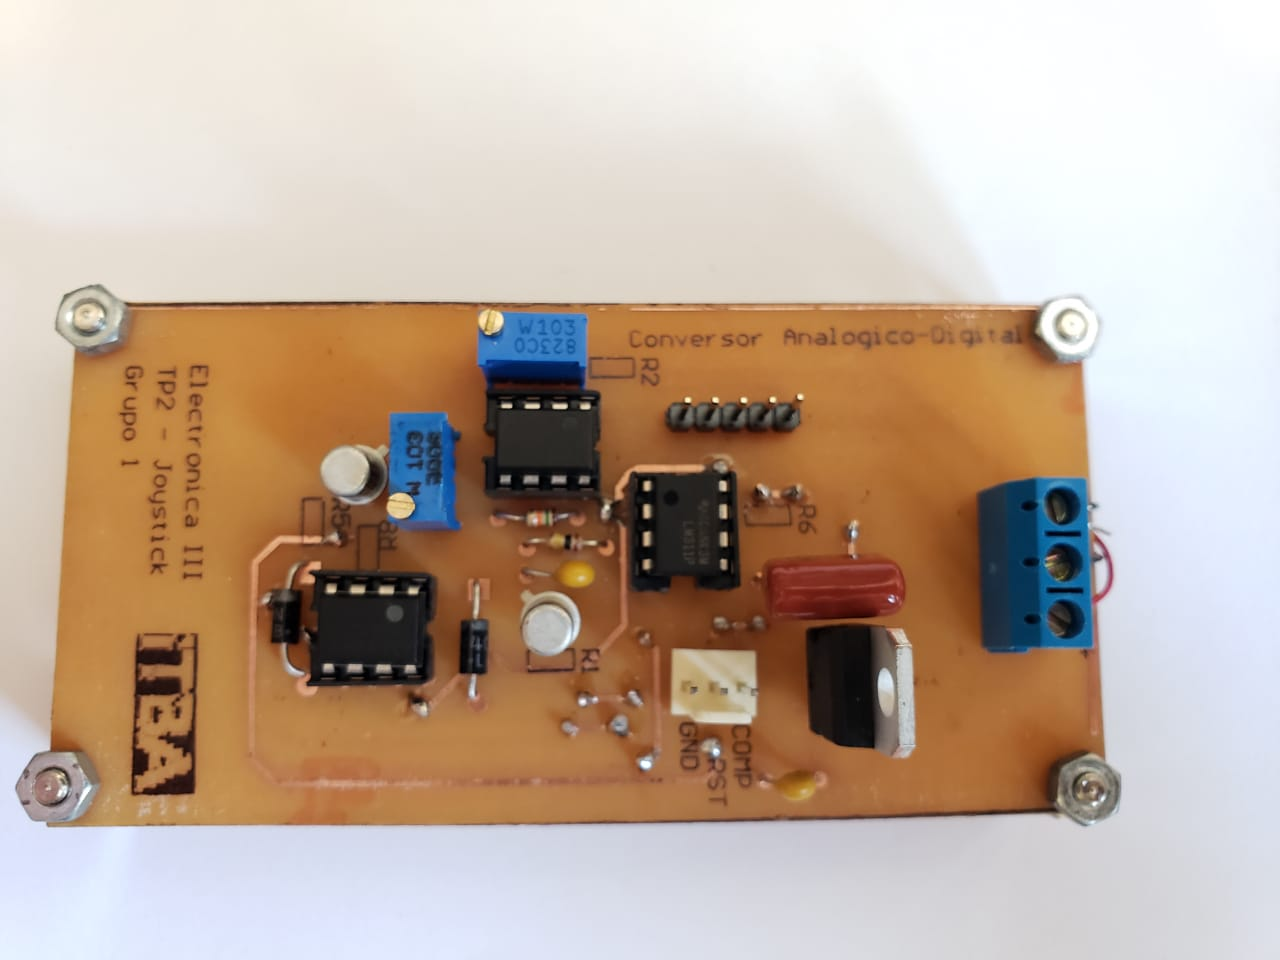
\includegraphics[width=0.5\textwidth]{../EJ8/Recursos/ANALOG_PCB}
    \caption{PCB del DAC utilizado para las pruebas.}
    \label{fig:PCB_ANALOG}
\end{figure}


\subsubsection{Contadores y memorias}
Como se menciona en la secci\'on anterior, para conocer la posici\'on del joystick es necesario contar la cantidad de pulsos que entran en el espacio teporal entre el comienzo de la rampa y cuando esta alcanza el nivel de tensi\'on en el joystick. Por esto es necesario tener un contador, en particular un contador que cuente hasta 100 en la duraci\'on de un per\'iodo de la se\~nal rampa. Adem\'as como es necesario mostrar la posici\'on en un display es importante que lo que se muestre en el display sea un valor v\'alido y no un valor intermedio de la cuenta, por esta raz\'on se presenta la necesidad de utilizar alg\'un tipo de memoria.


Como contador se decide utilizar un CD4518, un contador BCD de dos d\'igitos, ya que esto permite convertir el n\'umero de la cuenta a codificaci\'on 7 segmentos, el tipo de display utilizado. Este contador reinicia su cuenta cuando recibe el pulso de RESET, mencionado en la secci\'on anterior.

Para la memoria, se utiliza un 74HC123, Flip-Flop D \'octuple,  con su clock conectado a la salida del comparador, de manera que solo se actualice la salida de este cuando la cuenta esta finalizada. 

Se puede observar en la Figura \ref{fig:LOGIC_PCB} el respectivo PCB utilizado para las pruebas.
\begin{figure}[H]
    \centering
    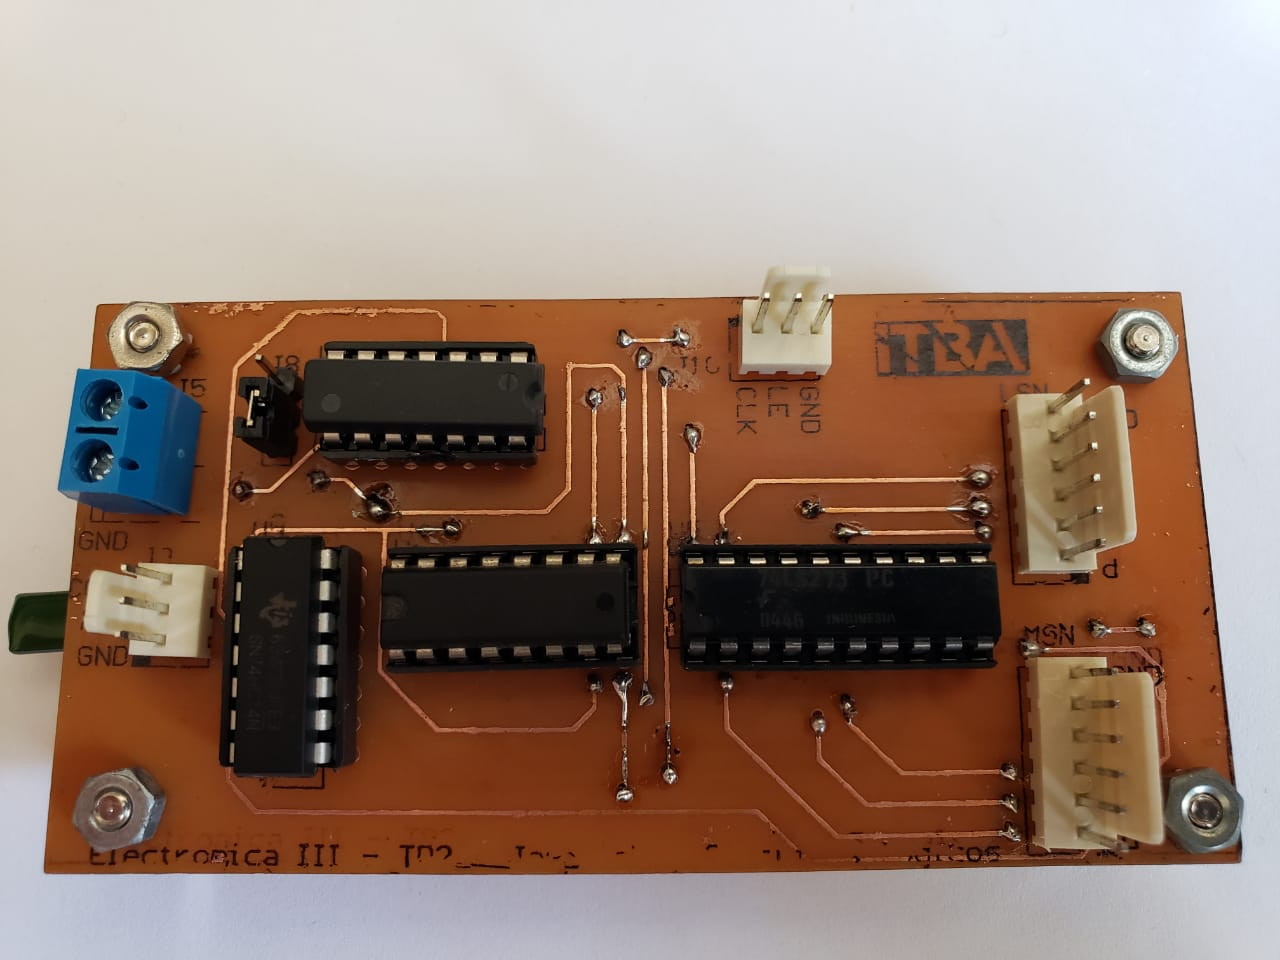
\includegraphics[width=0.5\textwidth]{../EJ8/Recursos/DIGITAL_PCB}
    \caption{PCB l\'ogico utilizado para las pruebas.}
    \label{fig:LOGIC_PCB}
\end{figure}

\subsubsection{Drivers y displays}

La interfaz del circuito son dos displays de siete segmentos, pudiendo representar su conjunto n\'umeros de cero a cien. La informaci\'on llega al m\'odulo de displays en forma de n\'umero binario en formato BCD, de forma separada para cada d\'igito. Esta informaci\'on es enviada a un decodificador de BCD a siete segmentos, cuya salida se conecta a cada uno de los displays.


Para controlar la tasa de refresco se emplea un clock proveniente de su respectivo m\'odulo, que opera sobre el \textit{Latch Enable (LE)} enable de un Flip-Flop que se ubica a la entrada del decodificador. De esta forma, variando la frecuencia de dicho clock se afecta directamente la tasa de refresco.

Se muestra en la Figura \ref{fig:DISP_PCB} el  PCB utilizado para las pruebas.
\begin{figure}[H]
    \centering
    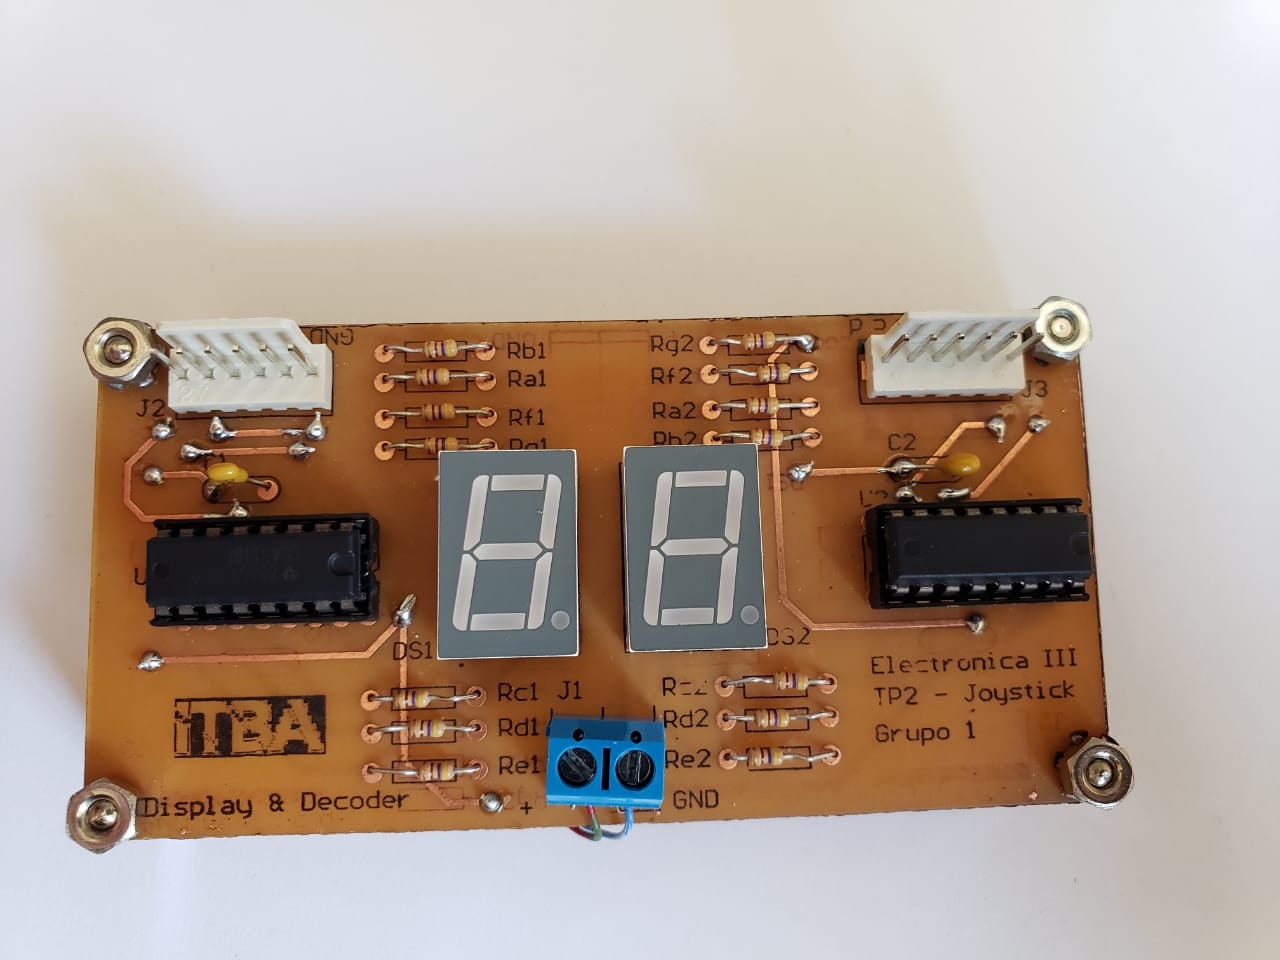
\includegraphics[width=0.5\textwidth]{../EJ8/Recursos/DISP_PCB}
    \caption{\label{fig:DISP_PCB}Se\~nales de inter\'es y salida del DAC}
\end{figure}

\subsubsection{Clocks}

El circuito posee en total dos se\~nales de clock. En primer lugar, uno de los clocks es el que comanda a la tasa de refresco de los display de siete segmentos. Esto se logra conectando el mismo al enable del latch que se encuentra previo a los display. La frecuencia de este clock oscila entre $1Hz$ y $20Hz$, aproximadamente.

Por otro lado, el segundo clock que integra el circuito es aquel que es utlizado para realizar el conteo que permite determinar la posici\'on del joystick. Idealmente, la frecuencia de dicho reloj debe ser tal que en un ciclo de rampa existan cien pulsos, de forma tal de limitar el valor m\'aximo del contador, y por ende discretizando la lectura de la posici\'on del joystick en ese valor.


Repecto a la implentaci\'on en circuito de ambos clocks, se emplea un integrado LM555 operando en modo astable para lograr la oscilaci\'on deseada. El circuito que se propone para tal fin se aprovecha de la carga y descarga de un capacitor para generar tal se\~nal, y se muestra a continuaci\'on.

\begin{figure}[H]
    \centering
    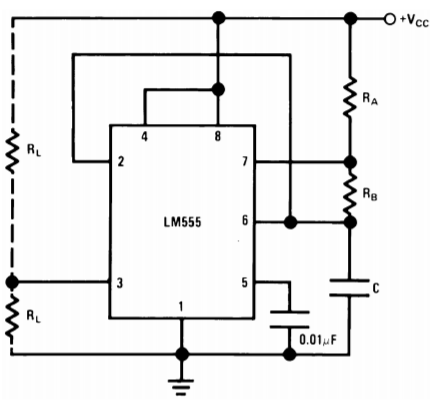
\includegraphics[width=0.5\textwidth]{../EJ8/Recursos/555_astable}
    \caption{\label{fig:ASTABLE_555}Oscilador astable - LM555}
\end{figure}

Asimismo los componentes determinan la frecuencia de oscilaci\'on del clock, respondiendo a la siguiente ecuaci\'on.

\begin{equation}
f_{clock} = \frac{1,44}{(R_A+2R_B)\cdot C}    
\end{equation}

Se realizaron los c\'alculos pertinentes y se seleccionaron los componentes, como se observa en la tabla de abajo.


  \begin{table}[H]
	\begin{center}
		\begin{tabular}{c c c c c}
		 Clock & Rango de frecuencias & $R_A$ & $R_B$ & $C$ \\
		\hline
		Refresh rate &$1Hz - 23Hz$ &$1 K\Omega (preset)$ & $100 \Omega$ & $180 nF$ \\
		Contador & $5KHz - 12KHz$ & $500 K\Omega$ (potenci\'ometro) & $180 \Omega$ & $4,7 \mu F$  
		\end{tabular}
		
		\caption{Componentes seleccionados}
	\end{center}
\end{table}

El resultado de la implementaci\'on en PCB se observa en la siguiente imagen.

\begin{figure}[H]
    \centering
    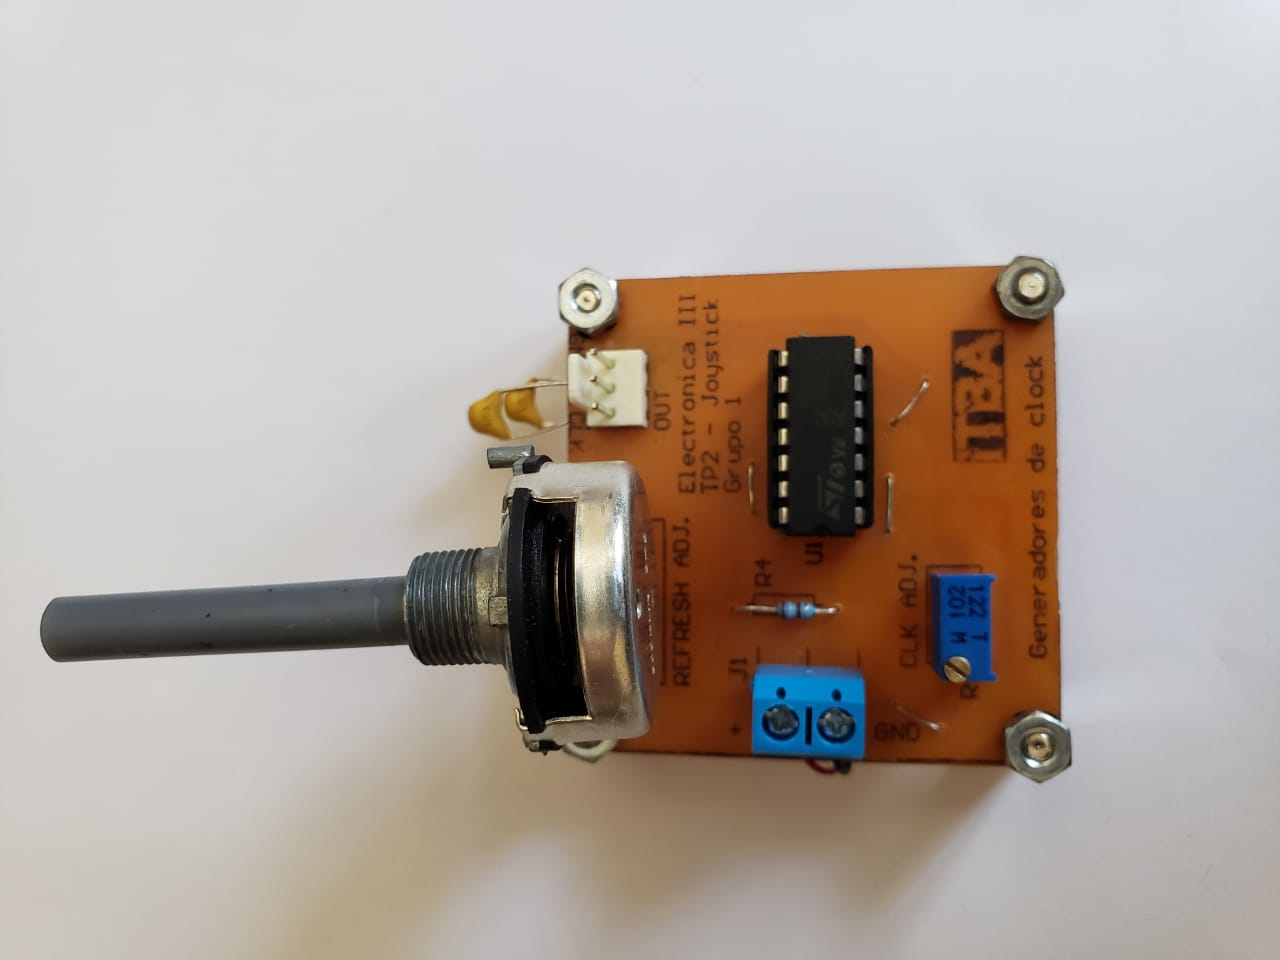
\includegraphics[width=0.7\textwidth]{../EJ8/Recursos/clocksPCB}
    \caption{\label{fig:BLOCK_DIAG}PCB de m\'odulo de clocks}
\end{figure}


\subsection{Funcionamiento y calibraci\'on}


Una vez implementado el circuito es necesario realizar una calibraci\'on del mismo, de modo tal que su funcionamiento sea el adecuado. En primer lugar, se deben calibrar tanto la frecuemncia de la rampa como la del clock asociado al contador. Habiendo fijado la frecuencia de la rampa en un determinado valor (en general, $5kHz$) mediante el ajuste del preset dedicado a tal fin, se procede a calibrar la frecuencia del clock del contador en un valor cien veces inferior a la frecuencia fijada. De esta forma se obtienen cien pulsos por cada ciclo de rampa. Por otro lado, es tambi\'en es necesario calibrar la amplitud de la rampa, estableciendo que el l\'imite superior de esta corresponda al m\'aximo valor de tensi\'on entregado a la salida del joystick.

Por \'ultimo, se var\'ia el potenci\'ometro que controla la tasa de refresco de los displays hasta que se llega al valor deseado.

\subsection{Problemas encontrados con la implementaci\'on}
Al momento de implemntar el sistema se pueden observar 3 problemas de relevancia.

El primero es que, al utilizar para la generaci\'on del clock un solo circuito integrado, la interferencia entre ellos era muy notoria, y perjudicaba al funcionamiento de la l\'ogica. Se colocan, con el fin de reducir esa interferencia al m\'inimo sin retardar los flancos del clock, lo que perjudicar\'ia a\'un m\'as el funcionamiento del sistema, capacitores de filtro entre los terminales de salida del generador de clocks.

El segundo, es que debido al alto valor de resistencia de los presets utilizados para la calibraci\'on de la sincron\'ia, el ajuste fino de este par\'ametro resulta dif\'icil y no se logra el funcionamiento perfecto del sistema. Por lo tant se sugiere que, como un criterio de dise\~no, se utilicen para lograr un ajuste m\'as preciso, presets de valor por lo menos un orden de magnitud menor que el preset utilizado, de forma de lograr un mejor ajuste y un mejor funcionamiento en general.

El tercero y \'ultimo, es la presencia de oscilaciones no deseadas, de menor amplitud que la se\~nal utilizada, en el flanco descendente de la se\~nal que se observa a la salida del comparador del DAC. Esta oscilaciones generan estados inv\'alidos o glitches en el Flip-Flop D, lo que provoca que se muestren cuentas intermedias en los displays. Para solucionar esto, se agregan compuertas NOT de tipo \textit{Schmitt trigger}, es decir que tienen un rango de tensiones m\'as amplio antes de pasar de estado bajo a alto y viceversa. Esto las hace m\'as insensibles al ruido y a estas oscilaciones, lo que mejora el funcionamiento.


\subsection{Conclusiones}
 Una conclusi\'on apreciable observada a lo largo del ejercicio es la diferencia entre los modelos te\'oricos y simulaciones respecto a los circuitos reales. En varios casos se apreciaron comportamientos no esperados en la respuesta del circuito, principalmente debido al ruido presente en el entorno de medici\'on. Para ello se debieron implementar soluciones tales como filtros para evitar esta situaci\'on.
